\begin{frame}
\titlepage
\end{frame}

\begin{frame}\frametitle{What is the article about ?}
  \begin{block}{Context}
    \begin{itemize}
    \item Portfolio of wind energy (can be solar)
    \item Liberalized electricity markets
  \end{itemize}
  \end{block}

  \begin{block}{Goals}
    \begin{itemize}
      \item Propose an operational trading strategy (\textit{based on the quantile of wind power production})
      \item Assess its performance
    \end{itemize}
  \end{block}
  \begin{block}{Inputs of the model}
    Forecasts of
    \begin{itemize}
      \item  Wind power production
      \item Spot market prices
      \item Imbalance prices (\textit{regulating market prices})
    \end{itemize}
  \end{block}
  \textit{Remark : Not a forecasting problem !}
\end{frame}


\begin{frame}\frametitle{What are the main assumptions ?}
\begin{block}{Assumptions}
\begin{itemize}
  \item Price-taker %(\textit{clearing price often below in the stack})
  % On fait un stack des differentes offre en fonction du prix est des quantités proposés
  % et on coupe à la demande (la demande fait le prix), on appelle ça le clearing price.
  % Nous on vendait souvent à 10 euros tandis que ça clear autour de 50. Il est arrivé
  % 2 fois que l'on est pas été exécuté.
  \item No practical limitations
  % totalement faux en suisse ou il ne supporte pas l'imbalance, sinon c'est
  %max du 40% règle implicite du marché sous peine de recevoir une lettre du
  % régulateur
  \item Don't care about the risk : only the long run matters , ie we may face
  severe losses on the short run
  % argent pas illimité, tu seras viré avant
  \item No curtailment % argument de tant que les prix sont positifs c'est pas
  %economiquement viable de curtailer sauf que c'est le TSO qui curtail et lui
  % il s'en fou de si c'est viable ou pas car ce qui l'interesse c'est de pas avoir
  % trop d'imbalance dans le systeme. D'autant plus que c'est un facteur important
  % a prendre en compte car si en italie l'imbalance du au curtailment est recompense
  % au prix du DA ce n'est pas le cas en allemagne, donc c'est un grand facteur de risque
  \item PTU (\textit{Program Time Units}) are independent : no market dynamic.
  % utile pour pouvoir les traités à part
  \item Imbalance volumes are never rewarded
  %je ne connais pas un marché ou ce soit vrai.
\end{itemize}
\end{block}
\end{frame}


\begin{frame}\frametitle{Notations}
  \begin{block}{Notations}
  \begin{itemize}
    \item $k$ : a specific PTU
    \item $\widetilde { W } _ { k }$ : amount of energy contracted in the spot market
    \item $W _ { k }$ : stochastic production of wind energy
    \item $\rho _ { k }$ : revenue
    \item $\rho _ { k } ^ { ( S ) }$ : revenue from spot
    \item $\rho _ { k } ^ { ( \uparrow / \downarrow ) }$ : revenue from balancing
    \item $\pi _ { k } ^ { ( S ) }$ : spot market price
    \item $\pi _ { k } ^ { ( \downarrow ) }$ : down-regulation price
    \item $\pi _ { k } ^ { ( \uparrow ) }$ : up-regulation price
  \end{itemize}
\end{block}

\end{frame}


\begin{frame}\frametitle{Some relations}
  \begin{block}{Relations that hold}

  \begin{itemize}
    \item $\rho _ { k } = \rho _ { k } ^ { ( S ) } + \rho _ { k } ^ { ( \uparrow / \downarrow ) }$
    \item $\rho _ { k } ^ { ( S ) } = \pi _ { k } ^ { ( S ) } \widetilde { W } _ { k }$
    \item $\rho _ { k } ^ { ( \uparrow / \downarrow ) } = \left\{ \begin{array} { l l } { \pi _ { k } ^ { ( \downarrow ) } \left( W _ { k } - \widetilde { W } _ { k } \right) , } & { W _ { k } \geq \widetilde { W } _ { k } } \\ { \pi _ { k } ^ { ( \uparrow ) } \left( W _ { k } - \widetilde { W } _ { k } \right) , } & { W _ { k } < \widetilde { W } _ { k } } \end{array} \right.$
    \item $\pi _ { k } ^ { ( \downarrow ) } \leq \pi _ { k } ^ { ( S ) }
    \leq \pi _ { k } ^ { ( \uparrow ) }$
  \end{itemize}
\end{block}

\end{frame}


\begin{frame}\frametitle{Reformulating the revenue}
  \begin{block}{Reformulating the revenue}

  \begin{itemize}
    \item $\rho _ { k } = \pi _ { k } ^ { ( S ) } W _ { k } + C _ { k } ^ { ( \uparrow / \downarrow ) }$
    \item $C _ { k } ^ { ( \uparrow / \downarrow ) } = \left\{ \begin{array} { l l } { \psi _ { k } ^ { ( \downarrow ) } \left( W _ { k } - \widetilde { W } _ { k } \right) , } & { W _ { k } \geq \widetilde { W } _ { k } } \\ { \psi _ { k } ^ { ( \uparrow ) } \left( W _ { k } - \widetilde { W } _ { k } \right) , } & { W _ { k } < \widetilde { W } _ { k } } \end{array} \right.$
    \item $\psi _ { k } ^ { ( \downarrow ) } = \pi _ { k } ^ { ( \downarrow ) } - \pi _ { k } ^ { ( S ) }$
    \item $\psi _ { k } ^ { ( \uparrow ) } = \pi _ { k } ^ { ( \uparrow ) } - \pi _ { k } ^ { ( S ) }$
  \end{itemize}
\end{block}

\begin{block}{Idea}
\begin{itemize}
  \item $\text{revenue} = \left(\text{term ind. from } \widetilde { W } _ { k }\right)
  + \left(\Delta \text{price } \cdot \Delta \text{imb. volumes}\right)$
\end{itemize}
\end{block}

\end{frame}


\begin{frame}\frametitle{Maximazing the revenue}
  \begin{block}{Expected Utility Maximization (EUM)}

  \begin{itemize}
    \item We want to find $\widetilde { W } _ { k } = \underset { \widetilde { W } _ { k } } { \arg \max } \mathbb { E } \left\{ \rho _ { k } \right\}$
   \item $\ldots$ which becomes $\widetilde { W } _ { k } = \underset { \overline { W } _ { k } } { \arg \max } \mathbb { E } \left\{ C _ { k } ^ { ( \uparrow / \downarrow ) } \right\}$
  \end{itemize}
\end{block}

\begin{block}{Reformulating $C _ { k } ^ { ( \uparrow / \downarrow ) }$}

  \begin{itemize}
    \item
$
  \mathbb { E } \left\{ C _ { k } ^ { ( \downarrow / \uparrow ) } \right\} = \underbrace{\int _ { 0 } ^ { + \infty } \int _ { 0 } ^ { \widetilde { W } _ { k } } \psi _ { k } ^ { ( \uparrow ) } \left( W _ { k } - \widetilde { W } _ { k } \right) d P _ { W _ { k } } d P _ { \psi _ { k } ^ { ( \uparrow ) } }}_{\widetilde { W } _ { k }\geq W_k \text{: short position}}$ $
+ \underbrace{\int _ { - \infty } ^ { 0 } \int _ { \widetilde { W } _ { k } } ^ { W ^ { ( m a x ) } } \psi _ { k } ^ { ( \downarrow ) } \left( W _ { k } - \widetilde { W } _ { k } \right) d P _ { W _ { k } } d P _ { \psi _ { k } ^ { ( 1 ) } }}_{\widetilde { W } _ { k }< W_k \text{: long position}}
$
  \end{itemize}
\end{block}
\end{frame}



\begin{frame}\frametitle{A stochastic optimization problem}
  \begin{block}{A stochastic optimization problem}

  \begin{itemize}
    \item Idea:  getting rid of $\psi _ { k } ^ { ( \downarrow ) }$ and $\psi _ { k } ^ { ( \uparrow ) }$
    \item $\mathbb { E } \left\{ C _ { k } ^ { ( \downarrow / \uparrow ) } \right\} = \widehat { \psi } _ { k } ^ { ( \uparrow ) } \int _ { 0 } ^ { W _ { k } } \left( W _ { k } - \widetilde { W } _ { k } \right) d P _ { W _ { k } }$
    $+\widehat { \psi } _ { k } ^ { ( \downarrow ) } \int _ { \widetilde { W } _ { k } } ^ { W ^ { ( m a x ) } } \left( W _ { k } - \widetilde { W } _ { k } \right) d P _ { W _ { k } }$
    \item $\ldots$ where $\widehat { \psi } _ { k } ^ { ( \uparrow ) }= \int _ { 0 } ^ { + \infty } \psi _ { k } ^ { ( \uparrow ) } d P _ { \psi _ { k } ^ { ( \uparrow ) } }$
    \item $\ldots$ and $\widehat { \psi } _ { k } ^ { ( \downarrow ) } = \int _ { - \infty } ^ { 0 } \psi _ { k } ^ { ( \downarrow ) } d P _ { \psi _ { k } ^ { ( \downarrow ) } }$
  \end{itemize}
\end{block}

\begin{block}{Remark}
  \begin{itemize}
    \item Are $\acc{\psi _ { k,t } ^ { ( \downarrow ) }}_t$ and
    $\acc{\psi _ { k,t } ^ { ( \uparrow ) }}_t$ stationary ?
  \end{itemize}
\end{block}
\end{frame}


\begin{frame}\frametitle{Solution of the SOP}
\begin{block}{Solution}
  \begin{itemize}
    \item $\widetilde { W } _ { k } = F _ { W _ { k } } ^ { - 1 } \left( \frac { \left| \widehat { \psi } _ { k } ^ { ( \downarrow ) } \right| } { \widehat { \psi } _ { k } ^ { ( \uparrow ) } + \left| \widehat { \psi } _ { k } ^ { ( \downarrow ) } \right| } \right)$
    \item $F _ { W _ { k } }$ cumulative distribution function of $W _ { k }$.
  \end{itemize}

  \begin{block}{Remark}
    \begin{itemize}
      \item A probabilistic forecast of $W_k$ is needed
    \end{itemize}
  \end{block}
\end{block}
\end{frame}


\begin{frame}\frametitle{Probabilistic forecast of $W_k$}
\begin{exampleblock}{Probabilistic forecast of production for a wind power portfolio in Eastern Denmark provided at 11 AM.}
  \begin{figure}
    \centering
      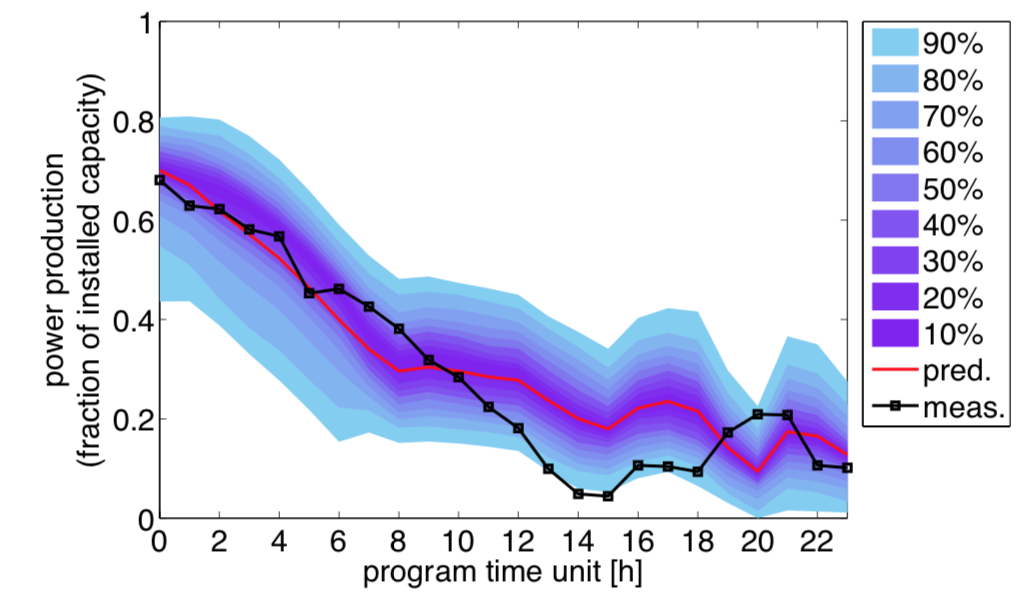
\includegraphics[width=0.9\textwidth]{Proba_forec}
  \end{figure}
\end{exampleblock}
\end{frame}


\begin{frame}\frametitle{How to compute unknown values ?}
\begin{block}{Estimators of unknown values}
  \begin{itemize}
    \item spot price: $\widehat { \pi } _ { k } ^ { ( S ) } = \mathbb { E } \left\{ \pi _ { k } ^ { ( S ) } \right\}$
    \item spread between spot and imbalance prices :
\begin{itemize}
  \item Down : $\widehat { \psi } _ { k \left| \psi _ { k } ^ { ( \downarrow ) } < 0 \right. } ^ { ( \downarrow ) } = \mathbb { E } \left\{ \psi _ { k } ^ { ( \downarrow ) } | \psi _ { k } ^ { ( \downarrow ) } < 0 \right\}$
  \item Up : $\widehat { \psi } _ { k \left| \psi _ { k } ^ { ( \uparrow ) } > 0 \right. } ^ { ( \uparrow ) } = \mathbb { E } \left\{ \psi _ { k } ^ { ( \uparrow ) } | \psi _ { k } ^ { ( \uparrow ) } > 0 \right\}$
\end{itemize}
  \end{itemize}
\end{block}

\begin{block}{Remark}
  \begin{itemize}
    \item $P _ { k } ^ { ( \downarrow ) } = P \left\{ \psi _ { k } ^ { ( \downarrow ) } < 0 \right\}$ and $P _ { k } ^ { ( \uparrow ) } = P \left\{ \psi _ { k } ^ { ( \uparrow ) } > 0 \right\}$ need to be computed
    \item $\ldots$ since $\widehat { \psi } _ { k } ^ { ( \downarrow ) } \neq \widehat { \psi } _ { k \left| \psi _ { k } ^ { ( \downarrow ) } <0\right. } ^ { ( \downarrow ) } $ but $\widehat { \psi } _ { k } ^ { ( \downarrow ) } = \widehat { \psi } _ { k \left| \psi _ { k } ^ { ( \downarrow ) } < 0 \right. } ^ { ( \downarrow ) }\cdot  {\color{red} P _ { k } ^ { ( \downarrow ) }}$
    \item $\ldots$ same for $\widehat { \psi } _ { k } ^ { ( \uparrow ) } \ldots$
  \end{itemize}
\end{block}
\end{frame}


\begin{frame}\frametitle{How to compute unknown values ?}
\begin{block}{Estimators of $P _ { k } ^ { ( \downarrow ) }$ and $P _ { k } ^ { ( \uparrow ) }$}
  \begin{itemize}
    \item $P _ { k } ^ { ( \downarrow ) } = P \left\{ \psi _ { k } ^ { ( \downarrow ) } < 0 \right\}$
    \item $P _ { k } ^ { ( \uparrow ) } = P \left\{ \psi _ { k } ^ { ( \uparrow ) } > 0 \right\}$
  \end{itemize}
\end{block}

\begin{exampleblock}{Example of forecast probabilities of up and down}
  \begin{figure}
    \centering
      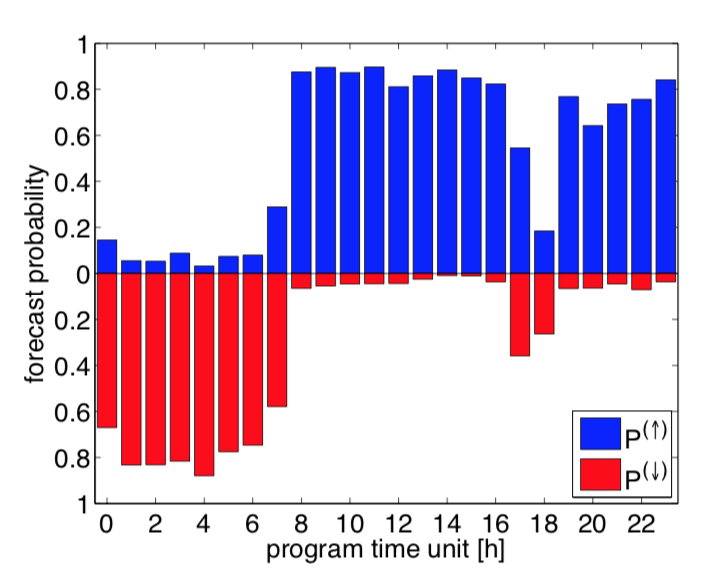
\includegraphics[width=0.5\textwidth]{saldo}
  \end{figure}
\end{exampleblock}
\end{frame}

\begin{frame}{Conclusion}
\begin{block}{A successful strategy ?}
  \begin{itemize}
  \item Simulation results show a PNL of $1OO$K euros /MW from the
  1st March 2008 to the 31st December 2008.
  \item not modeling its interaction with the system. An aggresive position can
  make the system switch $\ldots$
  \item Model improvements ?
  \begin{itemize}
    \item Imposing new constraints through a \textit{risk-aversion parameter}$\ldots$
    \item $\widetilde { W } _ { k } ^ { v , a _ { v } } = \min \left\{ \max \left\{ \widetilde { W } _ { k } , \widehat { W } _ { k } \cdot \left( 1 - a _ { v } \right) \right\} , \widehat { W } _ { k } \cdot \left( 1 + a _ { v } \right) \right\}$
    \item $\ldots$ where $a _ { v }\in \acc{0.1, 0.2}$
  \end{itemize}
  \end{itemize}
\end{block}
\end{frame}
